\title{Dynamic Programming}
\author{
        Benjamin Shih \\
        Simple Explanations\\
}
\date{Last updated: \today}

\documentclass[12pt]{article}
\usepackage{graphicx}

\begin{document}
\maketitle

\section{Prerequisites}
\begin{itemize}
\item Counting
\item Target Audience: 5
\end{itemize}

\section{An Explanation In Cookies}
Person A: ``Here, have a batch of cookies:''\\
\\
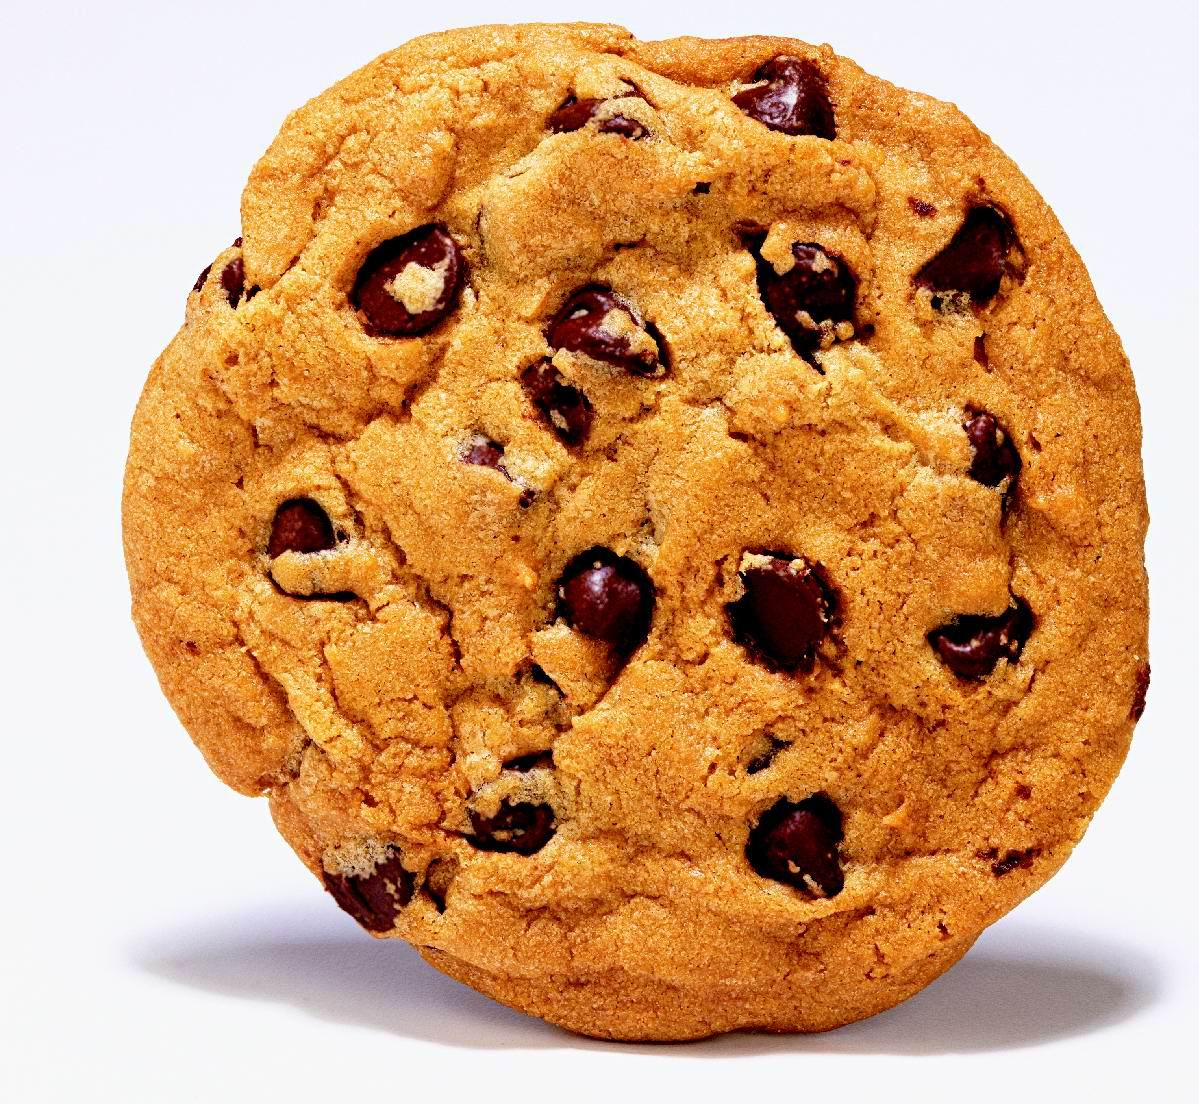
\includegraphics[height=10mm, width=10mm]{cookie.jpg}
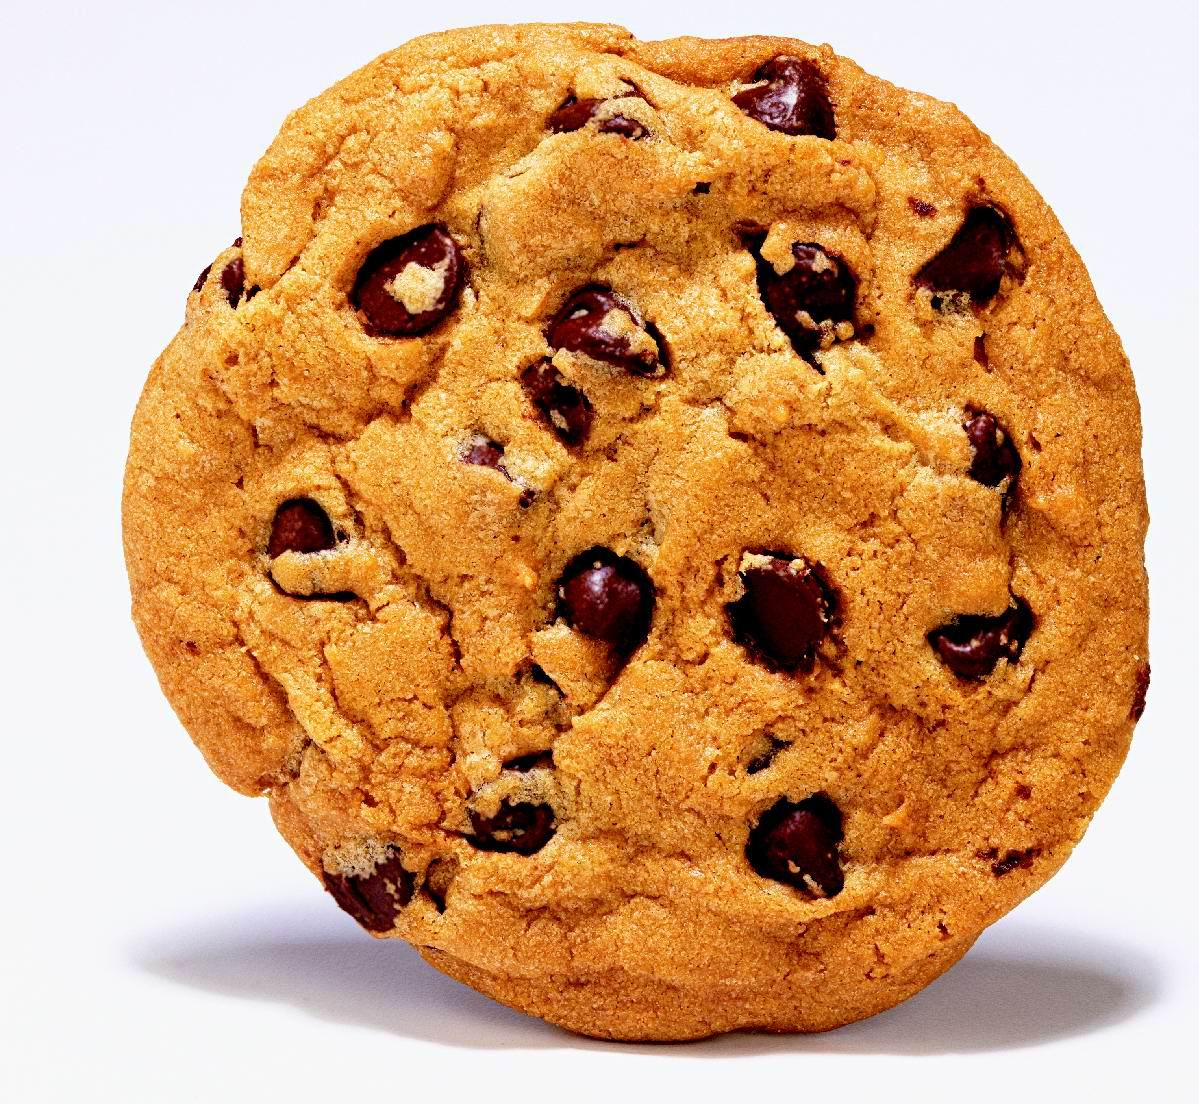
\includegraphics[height=10mm, width=10mm]{cookie.jpg}
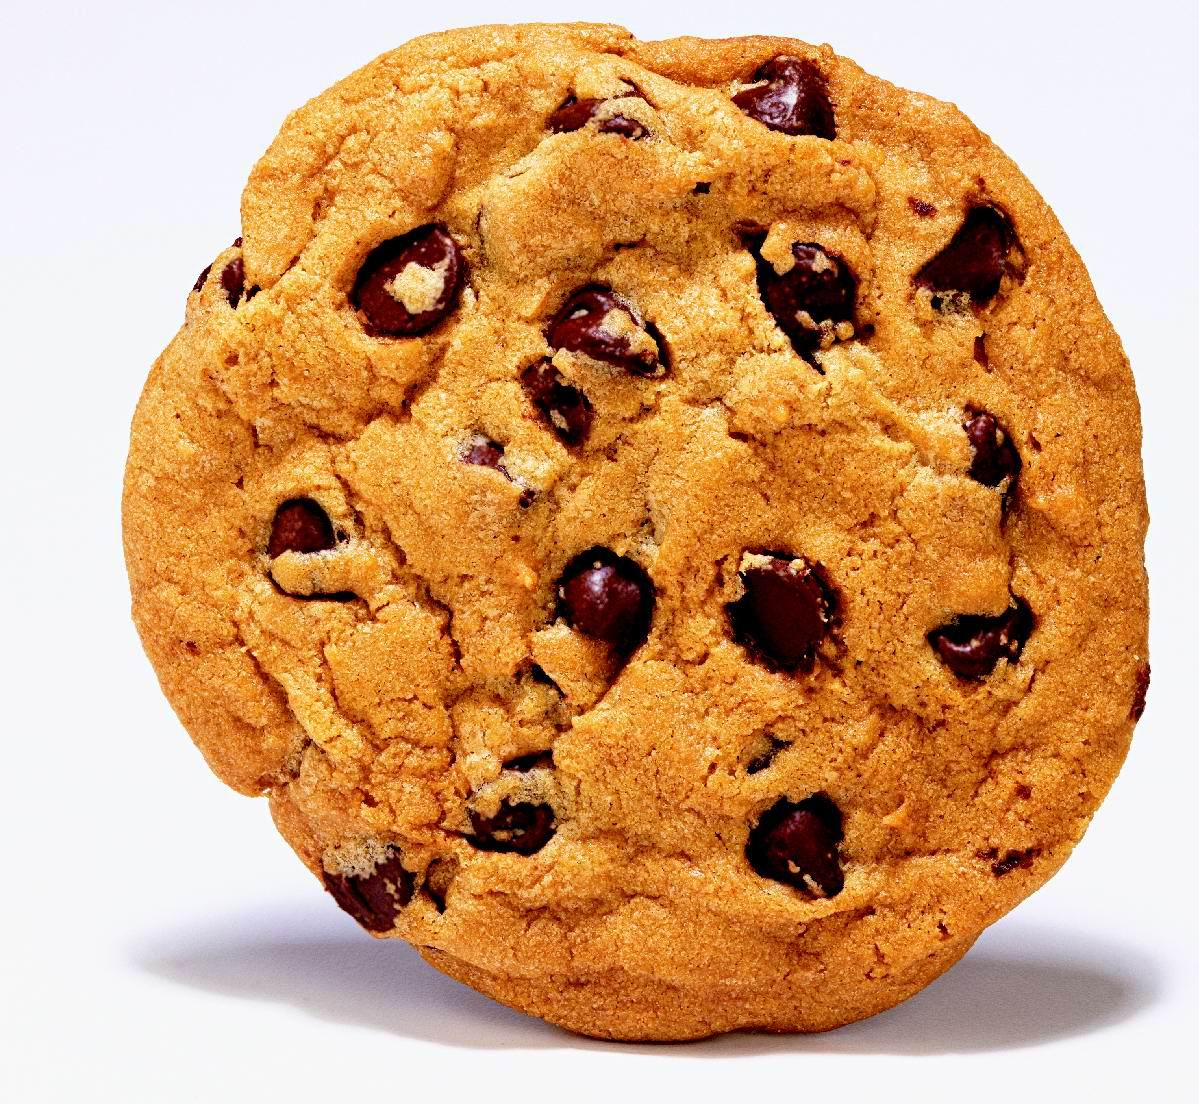
\includegraphics[height=10mm, width=10mm]{cookie.jpg}
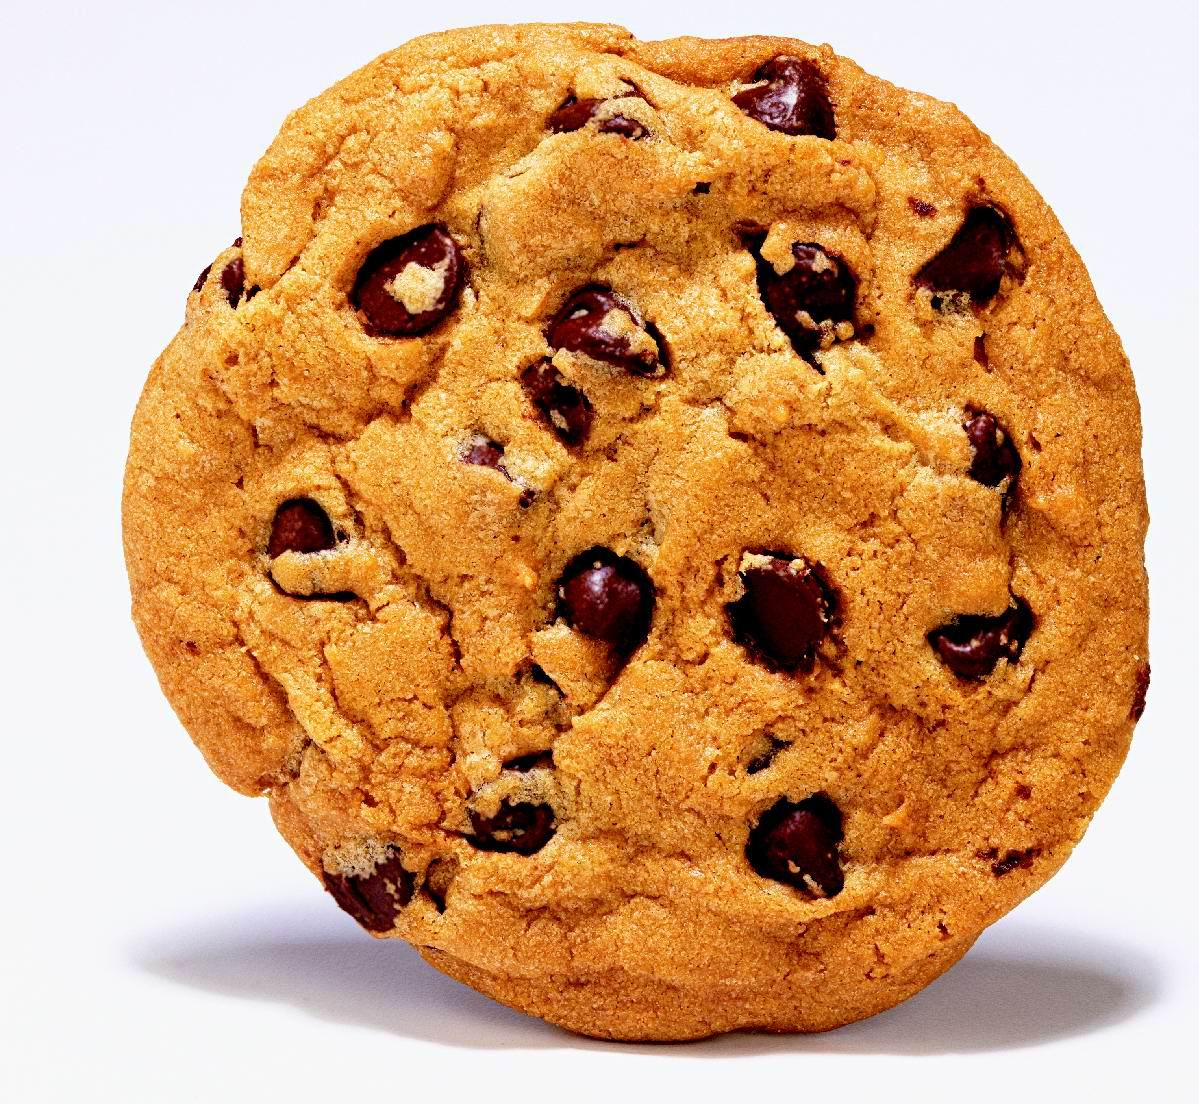
\includegraphics[height=10mm, width=10mm]{cookie.jpg}
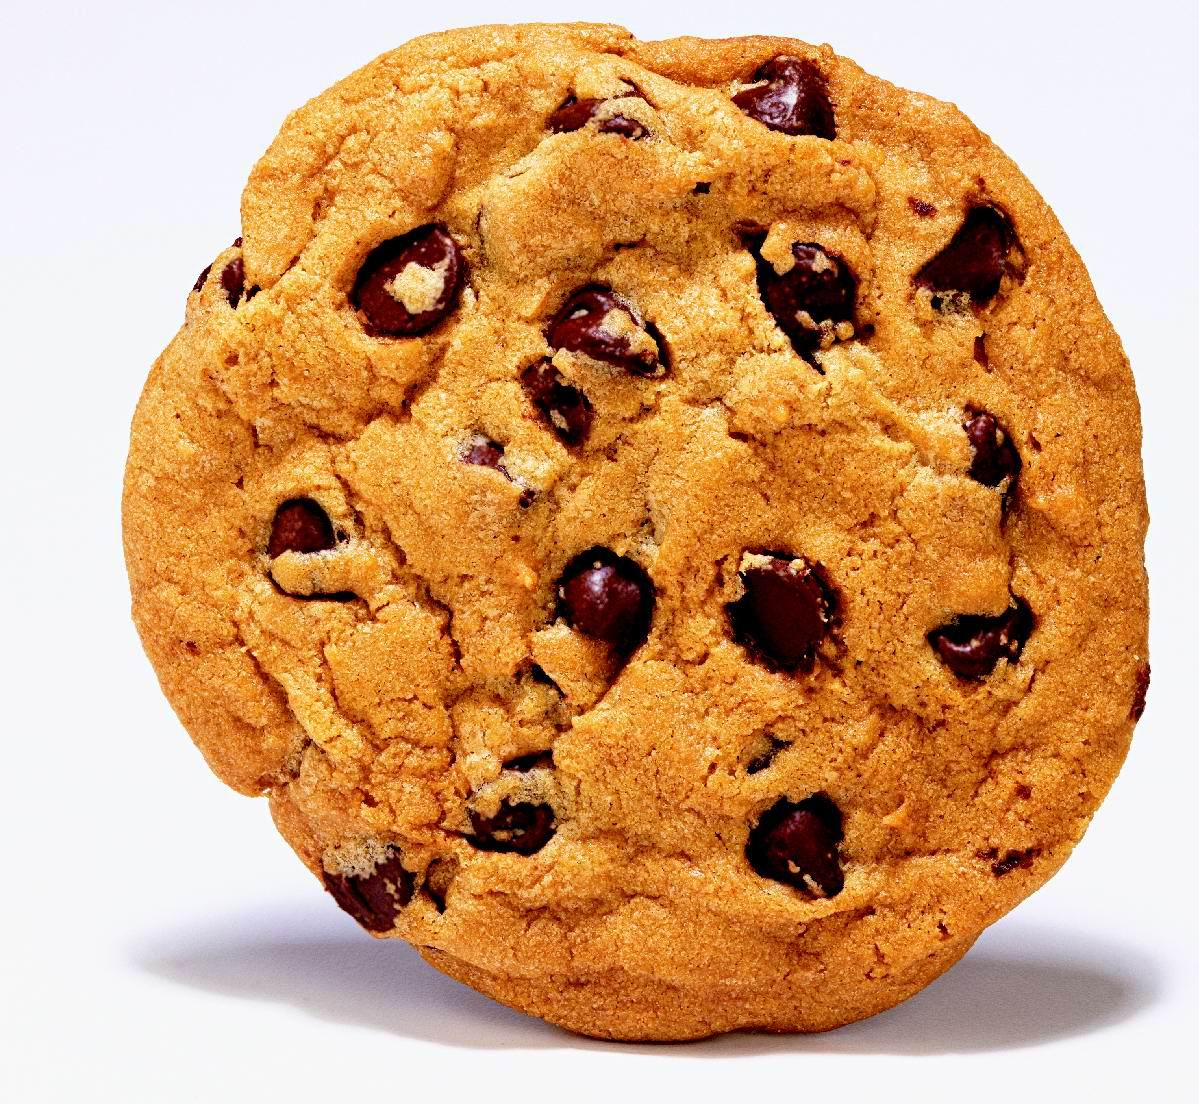
\includegraphics[height=10mm, width=10mm]{cookie.jpg}
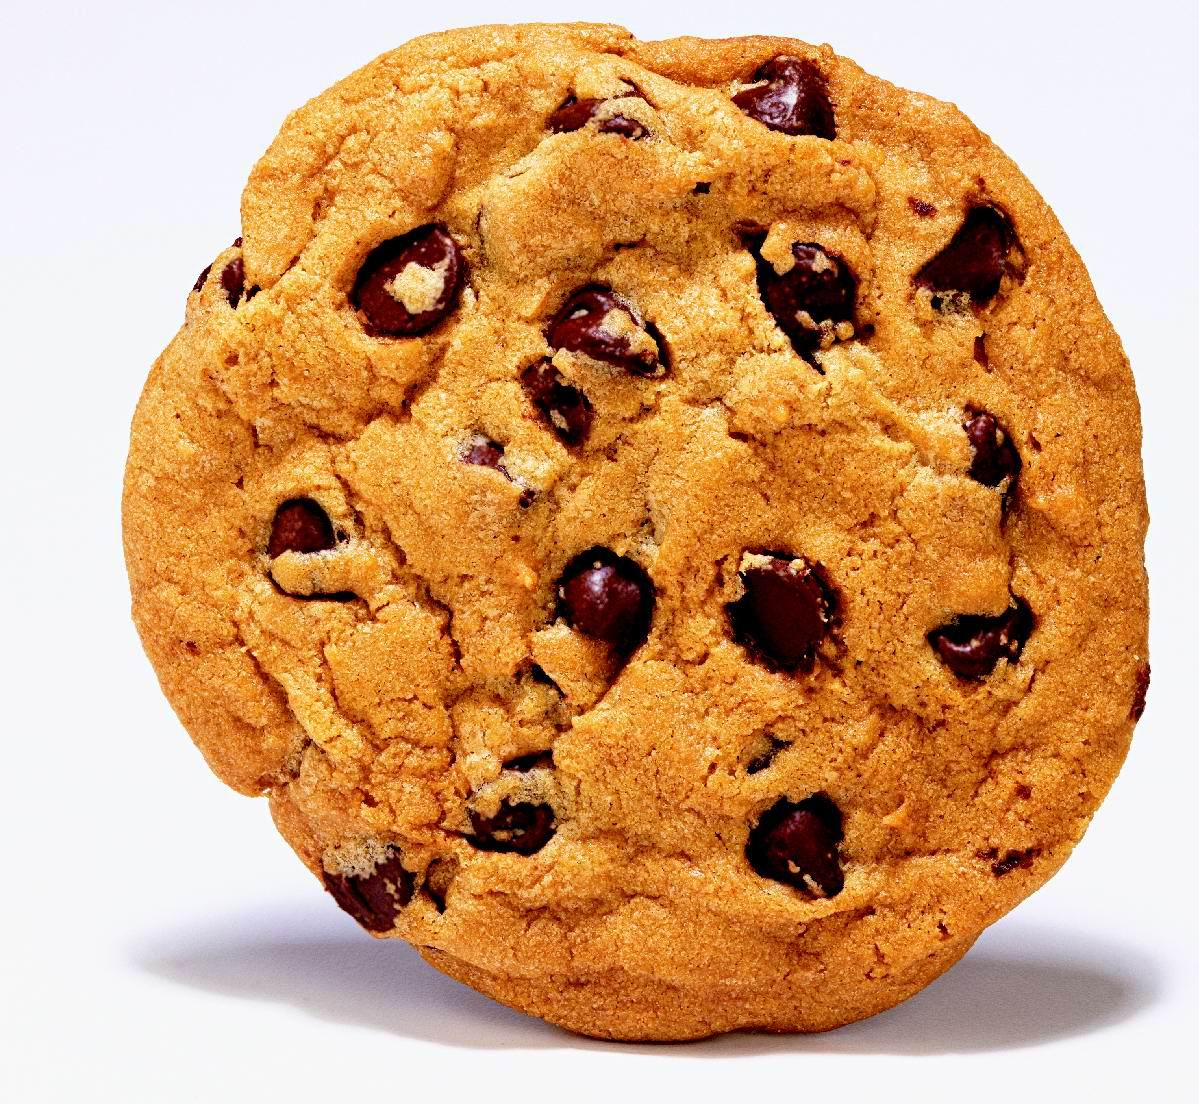
\includegraphics[height=10mm, width=10mm]{cookie.jpg}
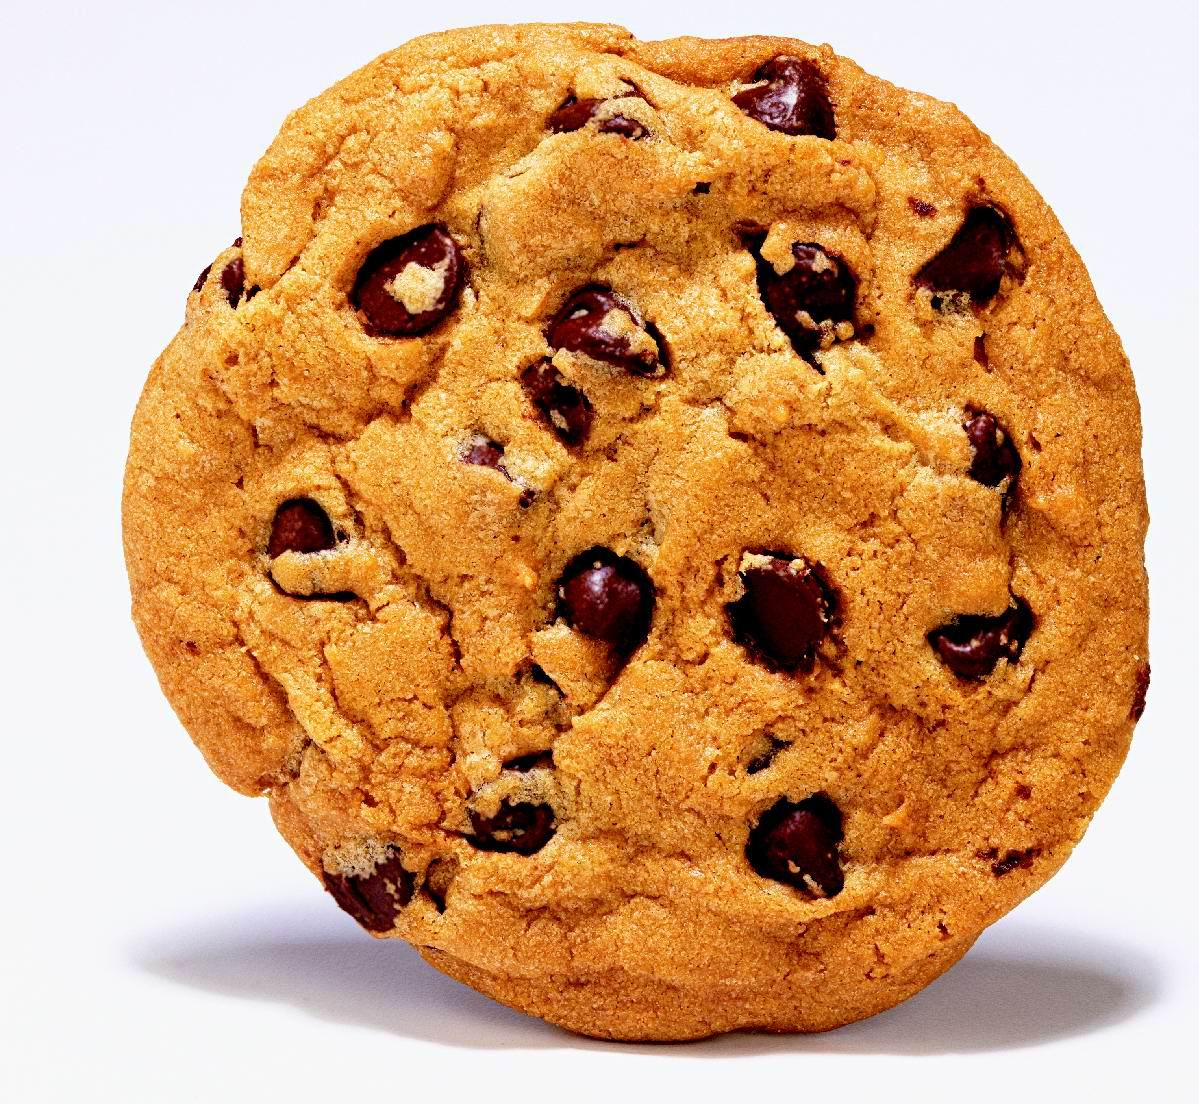
\includegraphics[height=10mm, width=10mm]{cookie.jpg}
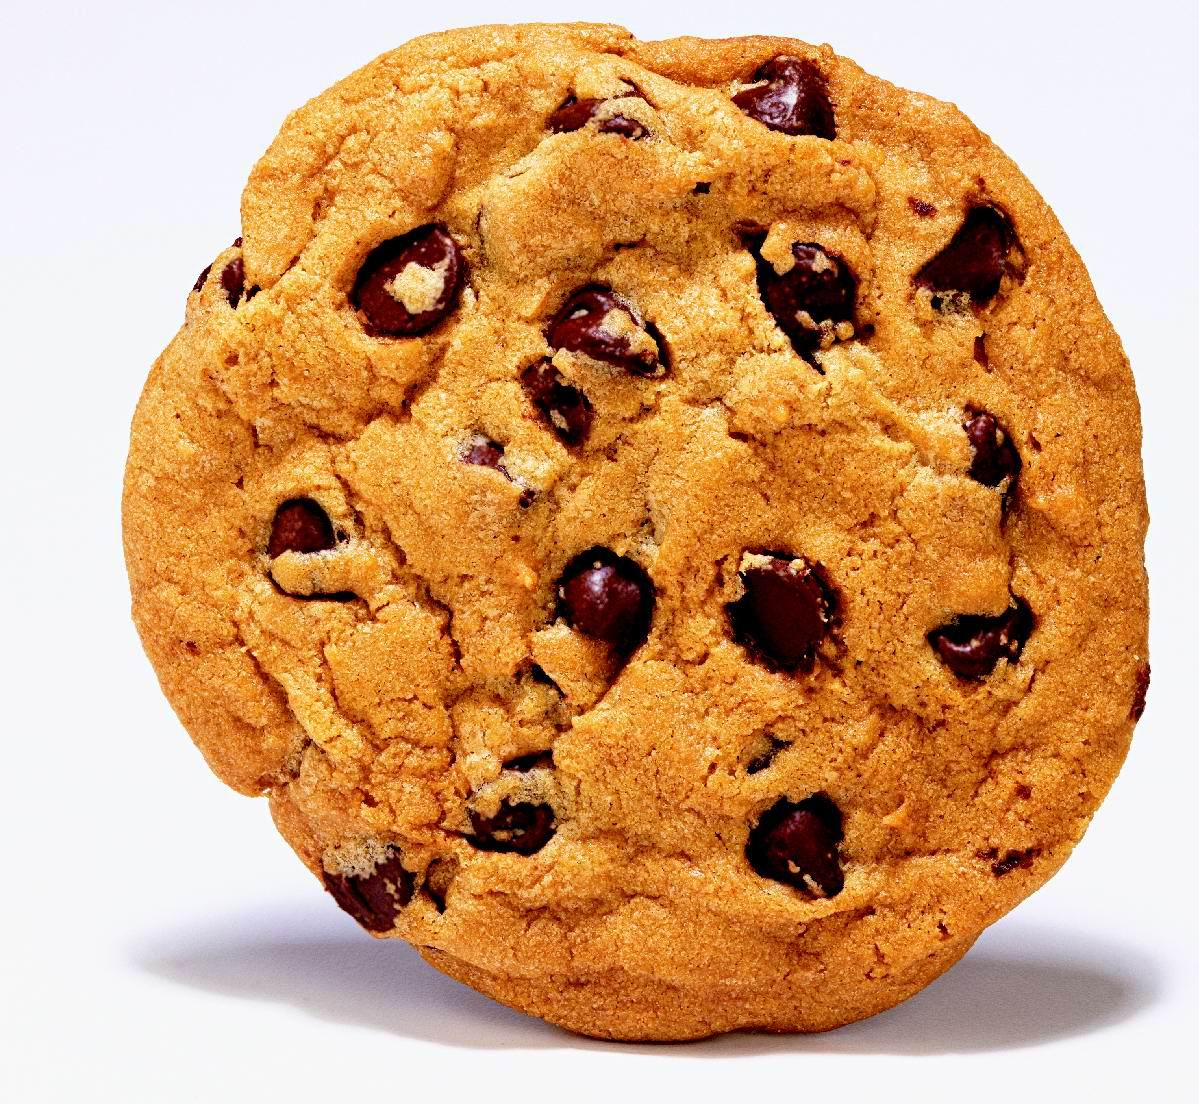
\includegraphics[height=10mm, width=10mm]{cookie.jpg}
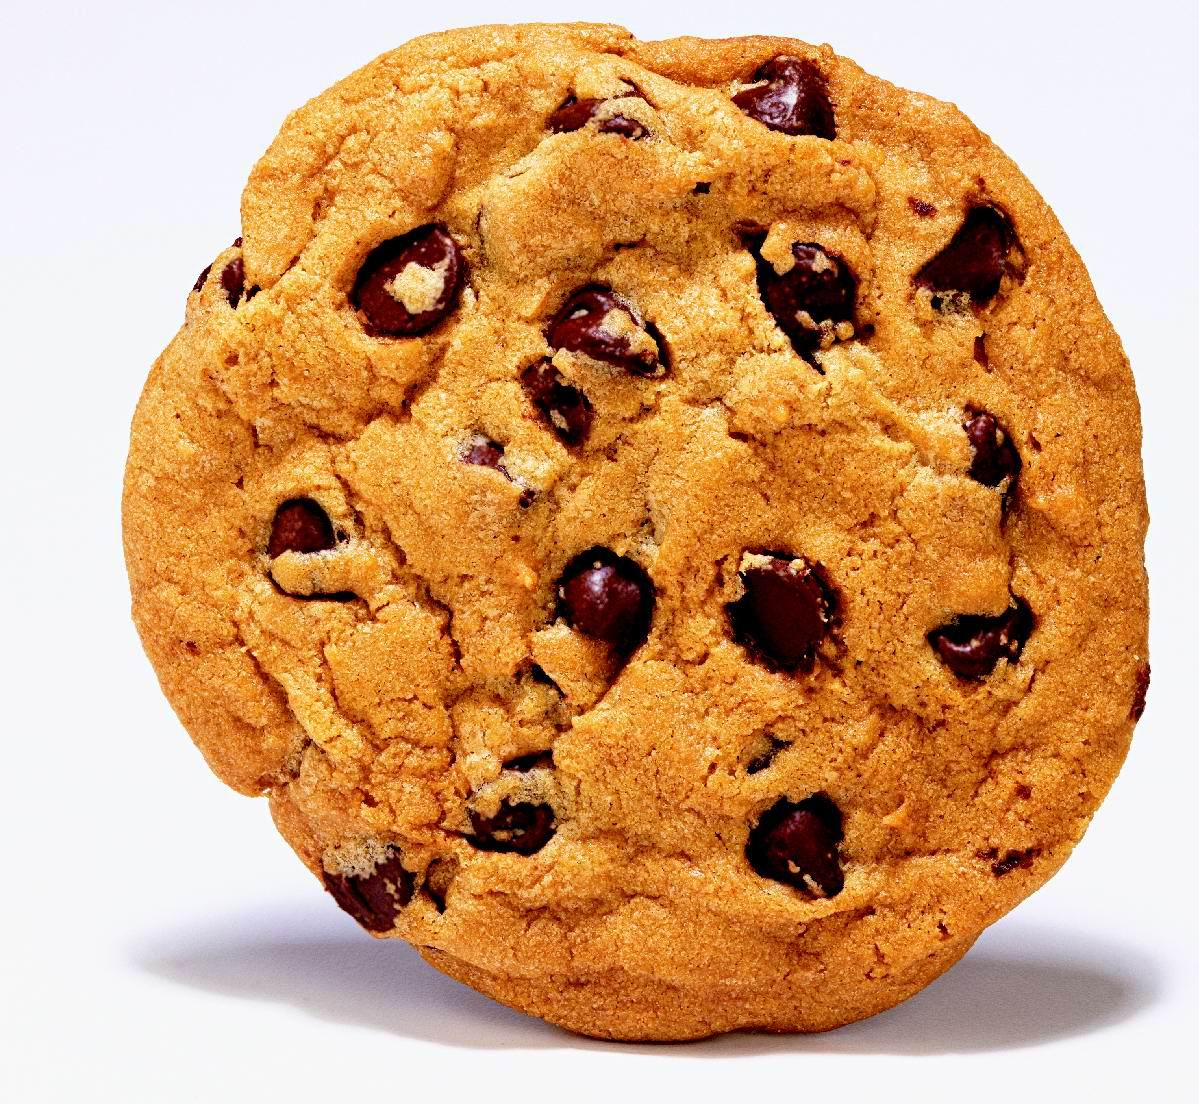
\includegraphics[height=10mm, width=10mm]{cookie.jpg}
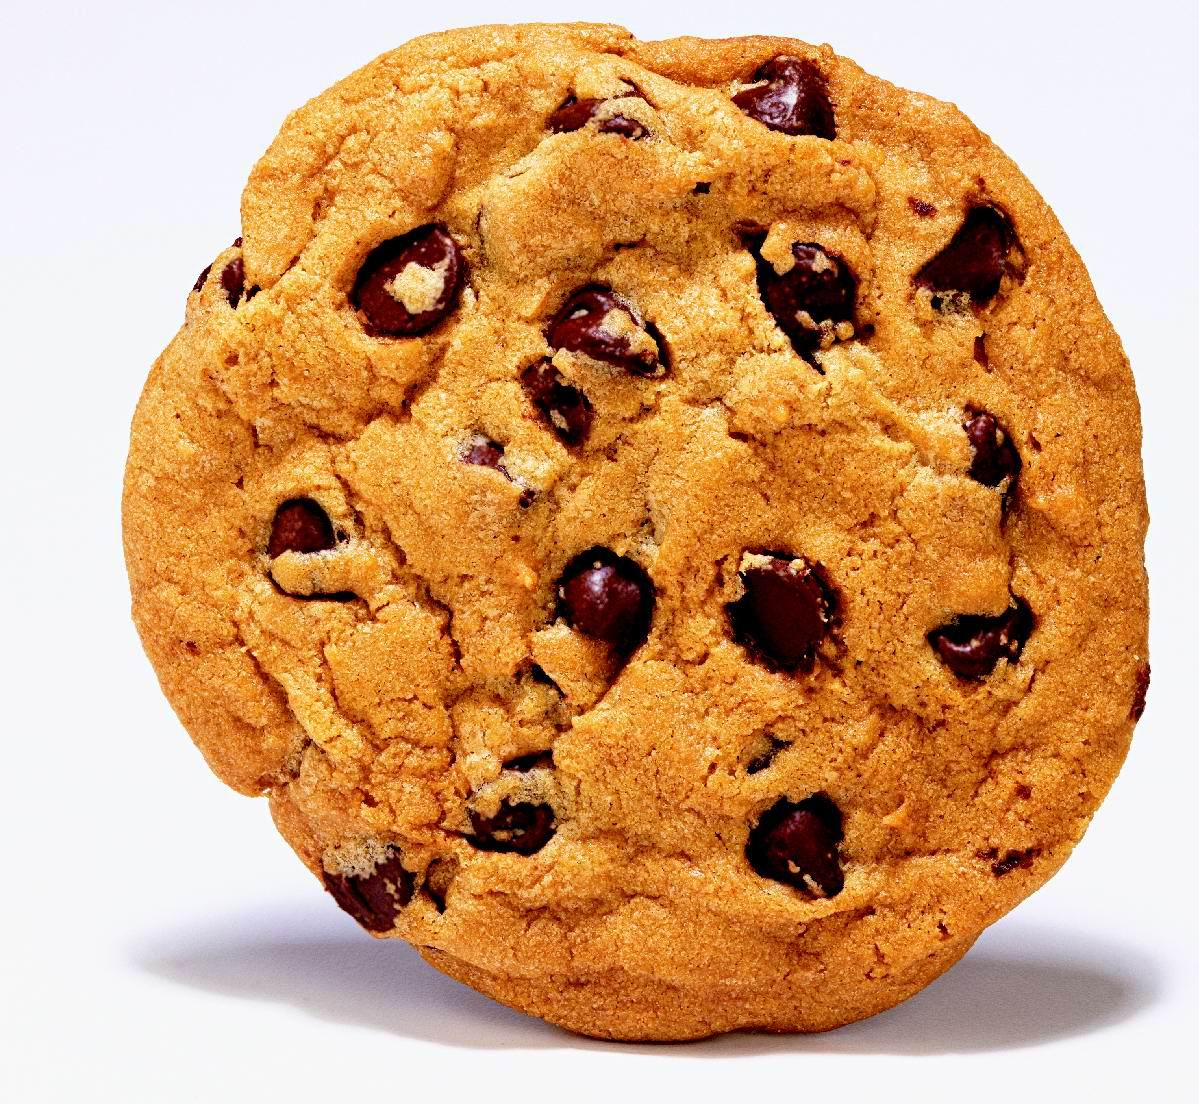
\includegraphics[height=10mm, width=10mm]{cookie.jpg}
\\
A: ``How many cookies did I give you?''\\
Person B: ``[counting...] You gave me 10 cookies.''\\
A: ``Here, have another batch of cookies:''\\
\\
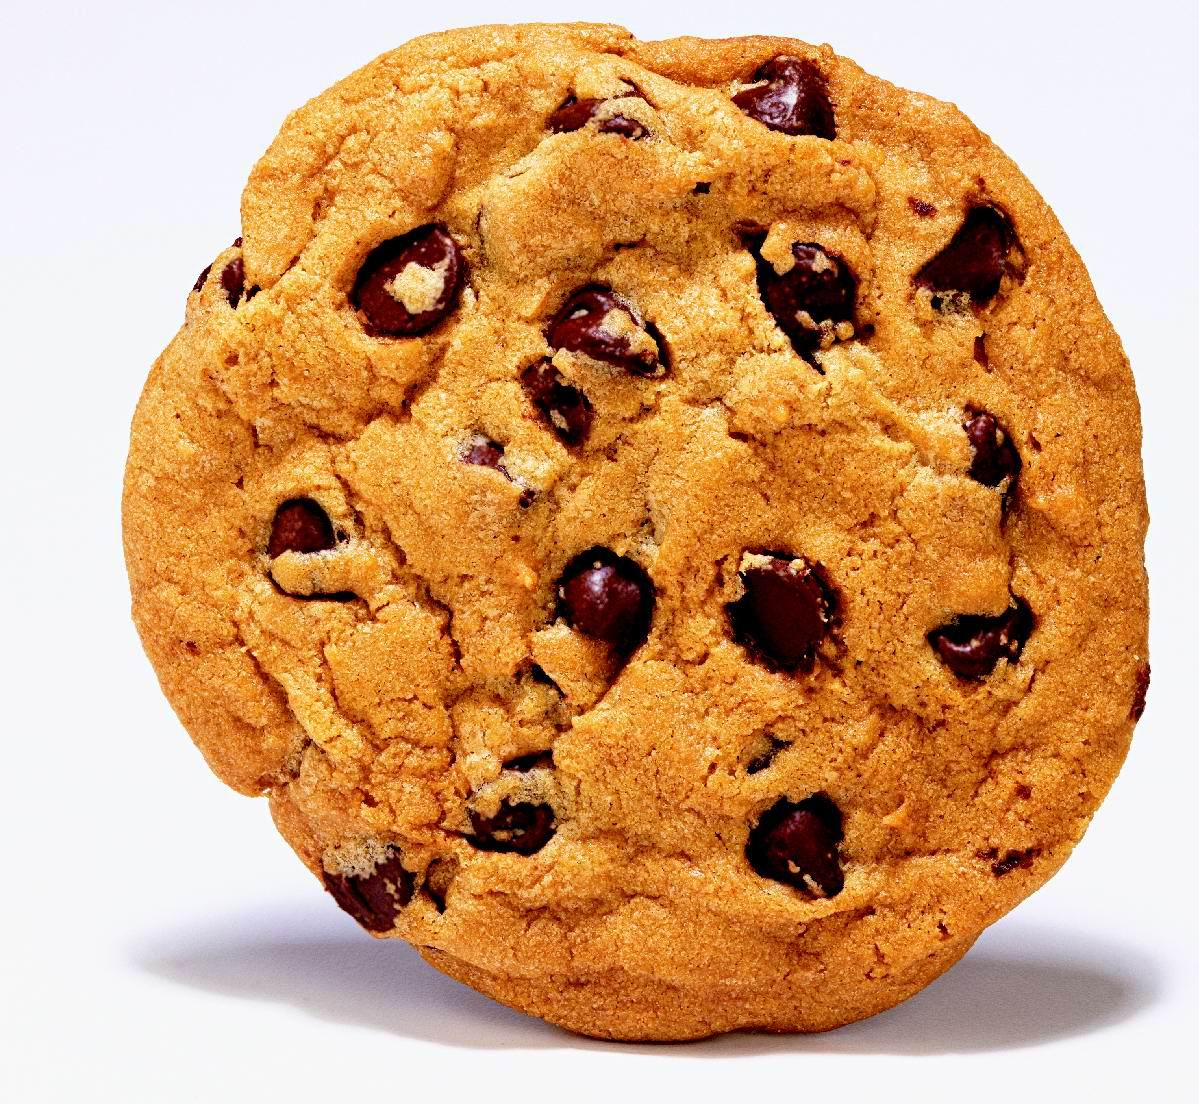
\includegraphics[height=10mm, width=10mm]{cookie.jpg}
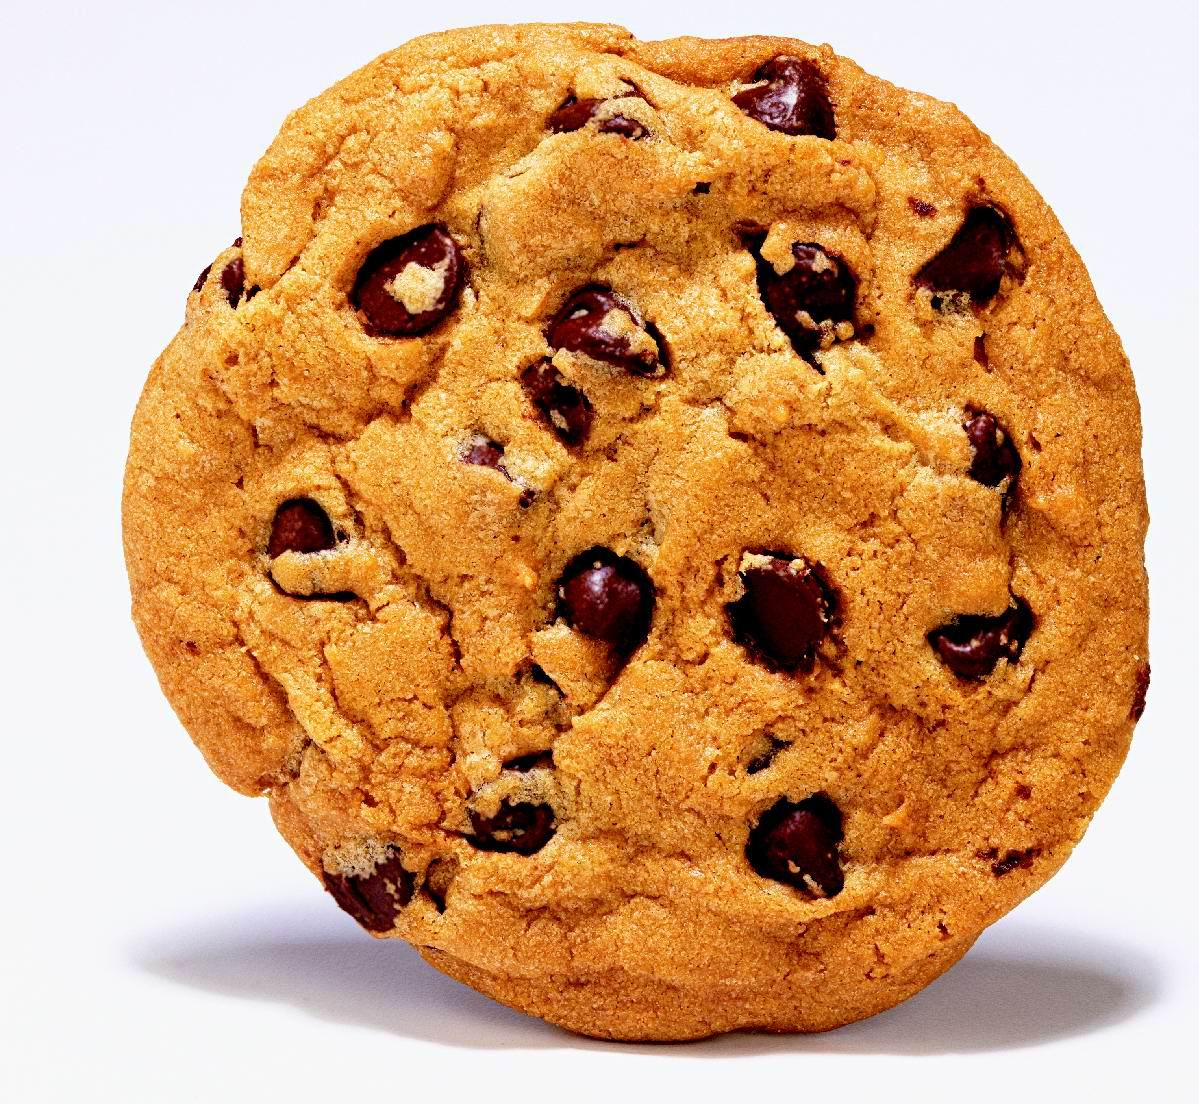
\includegraphics[height=10mm, width=10mm]{cookie.jpg}
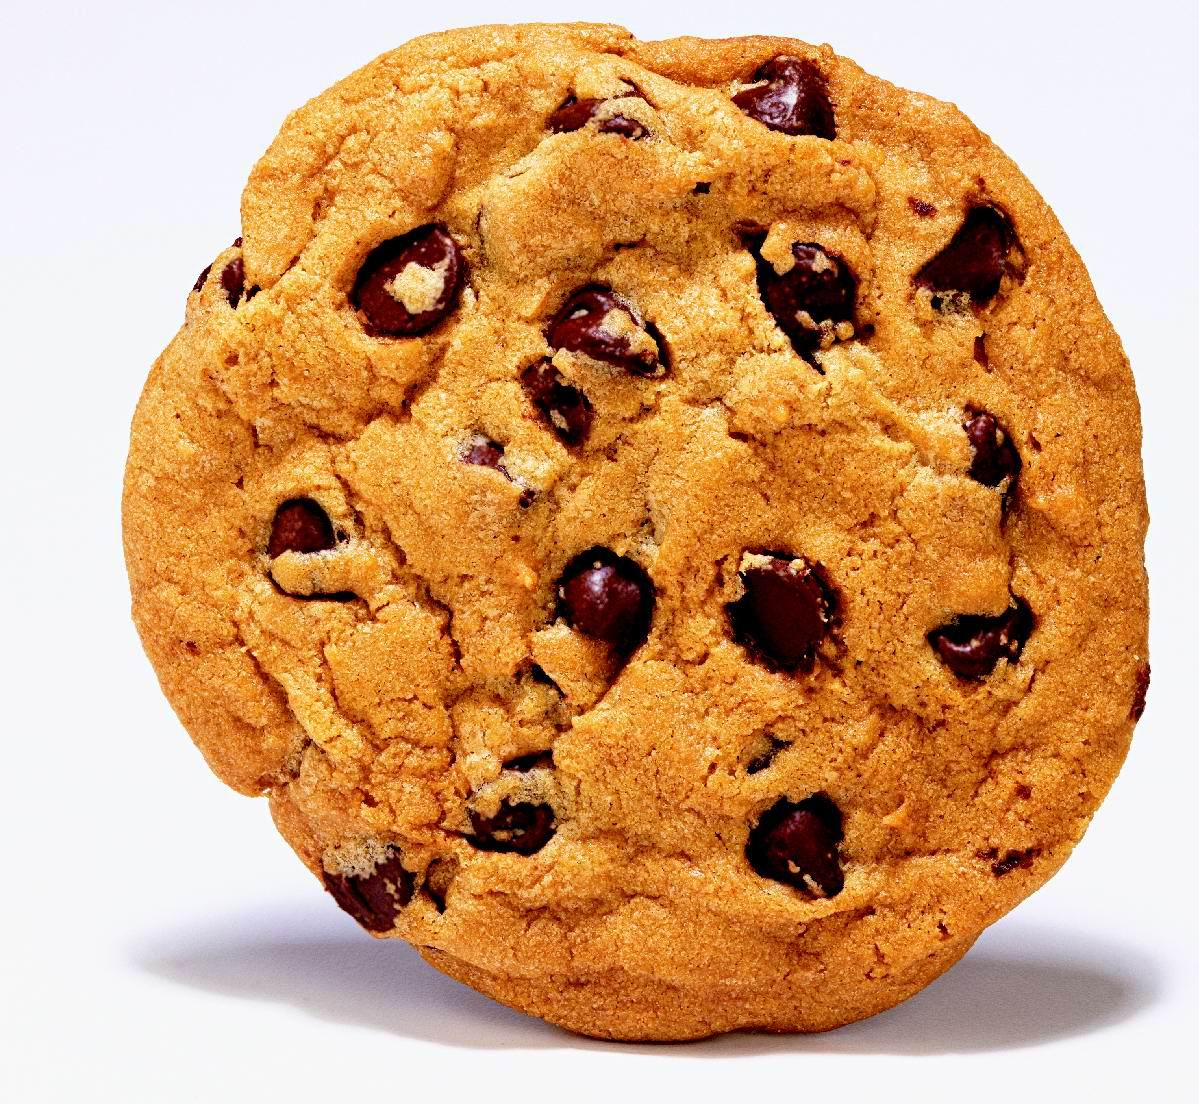
\includegraphics[height=10mm, width=10mm]{cookie.jpg}
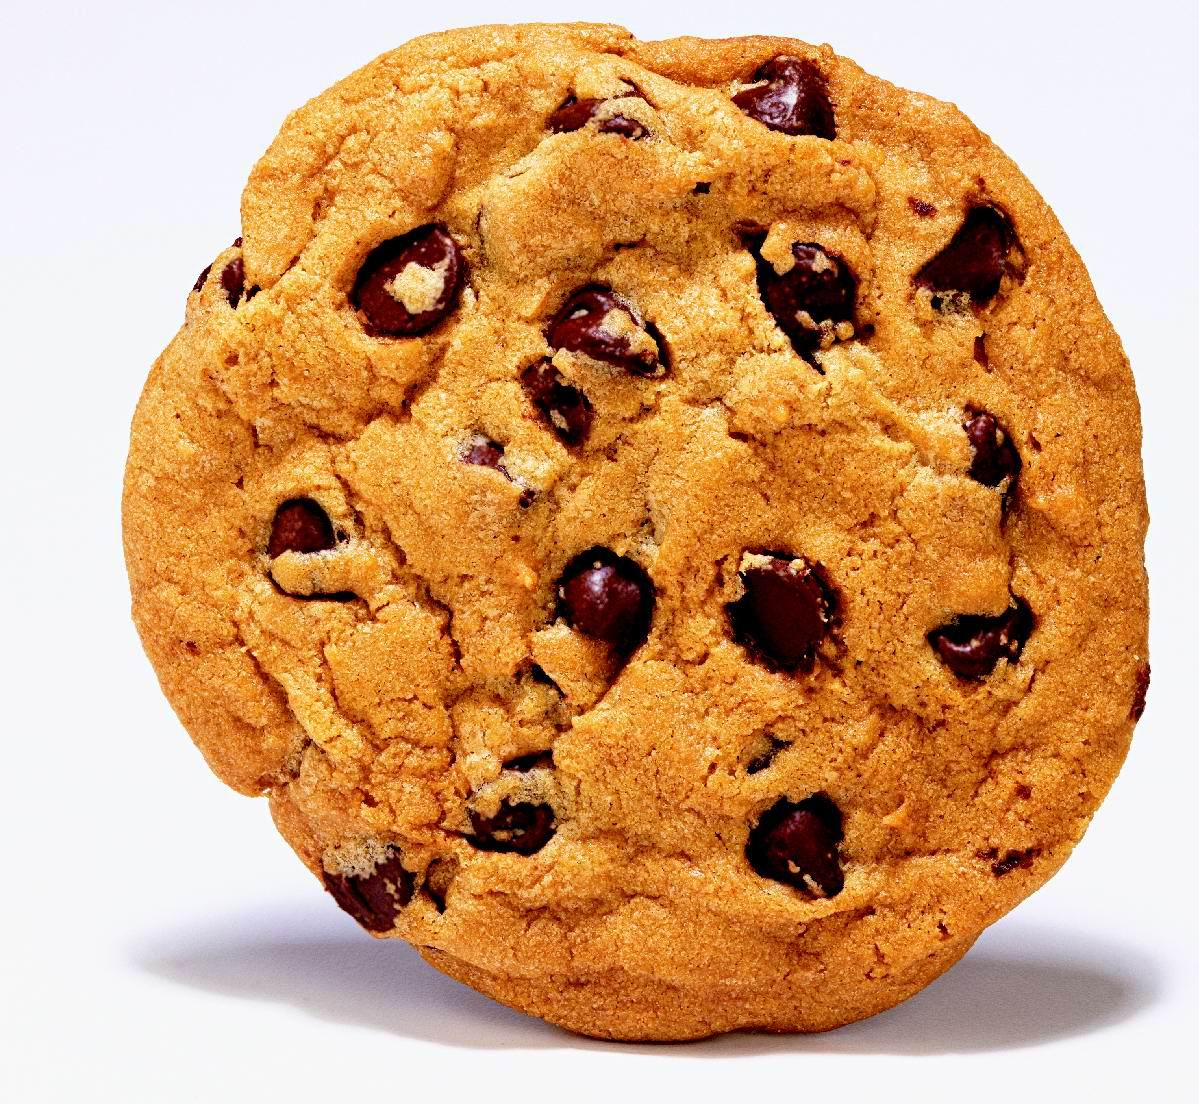
\includegraphics[height=10mm, width=10mm]{cookie.jpg}
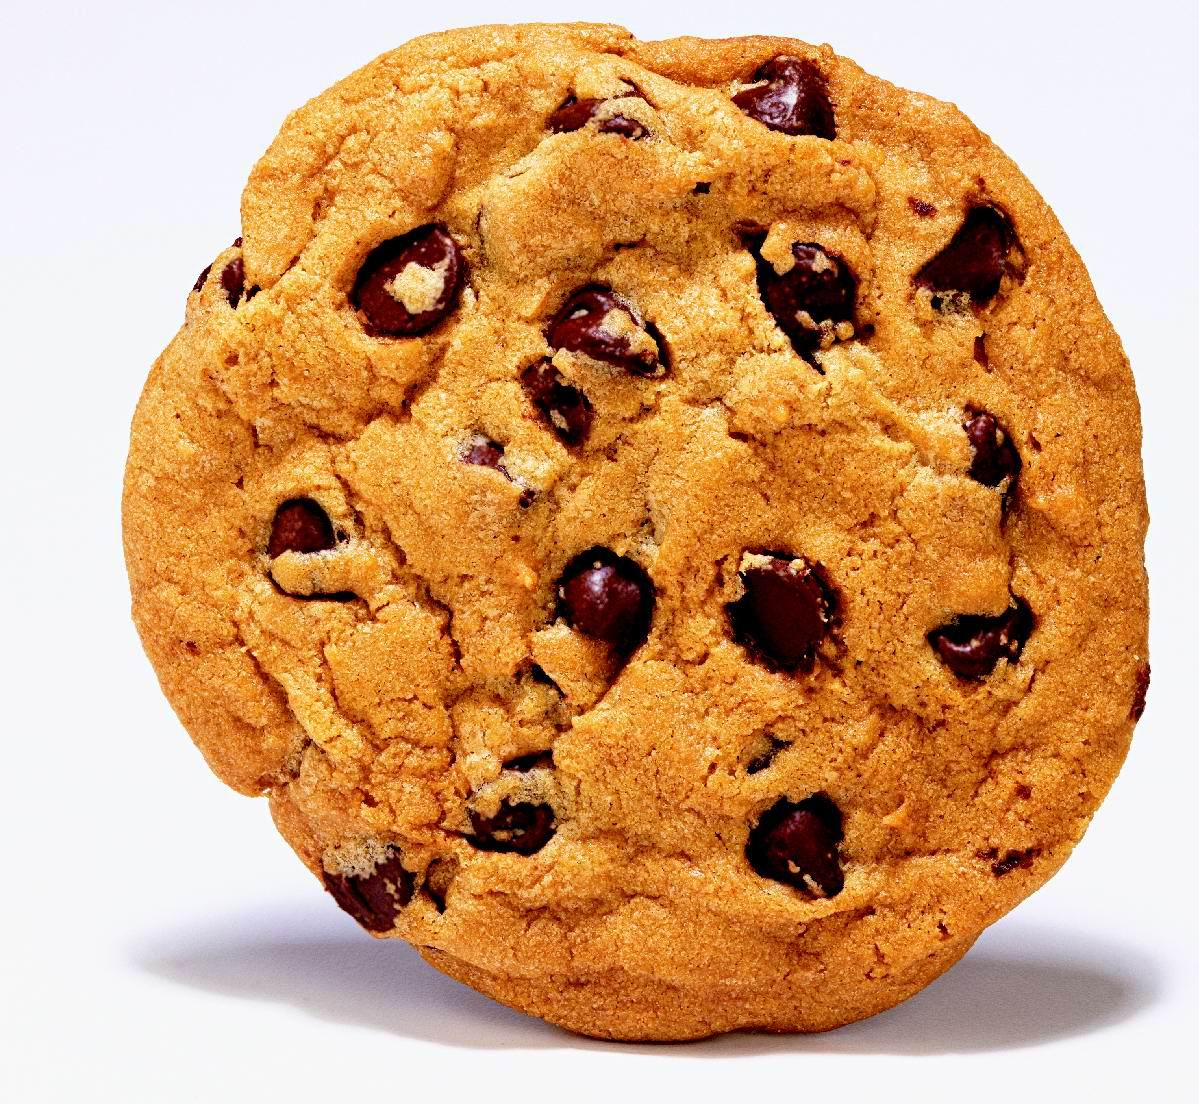
\includegraphics[height=10mm, width=10mm]{cookie.jpg}
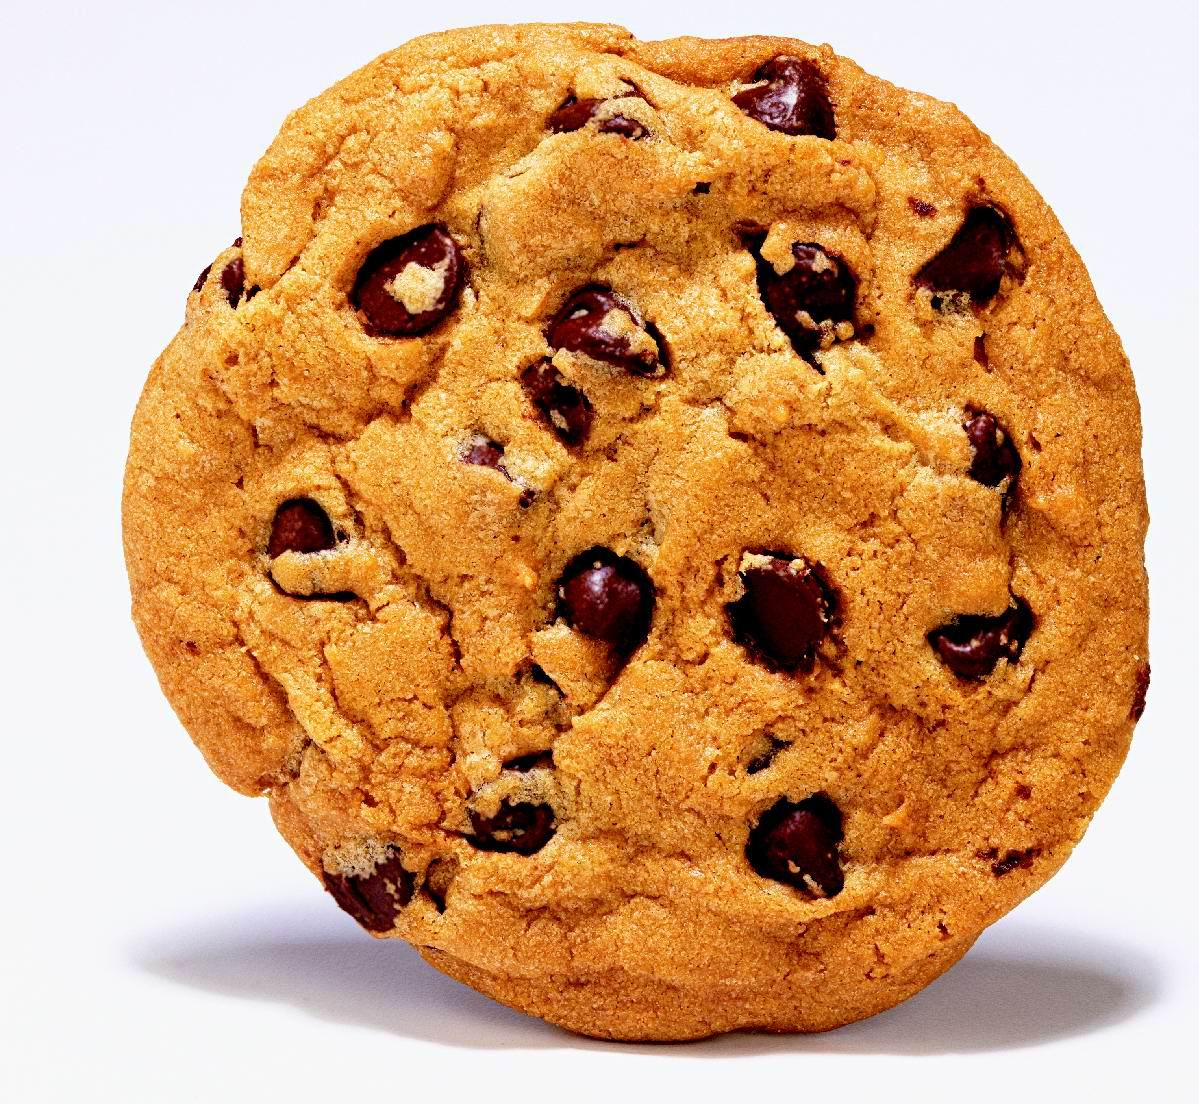
\includegraphics[height=10mm, width=10mm]{cookie.jpg}
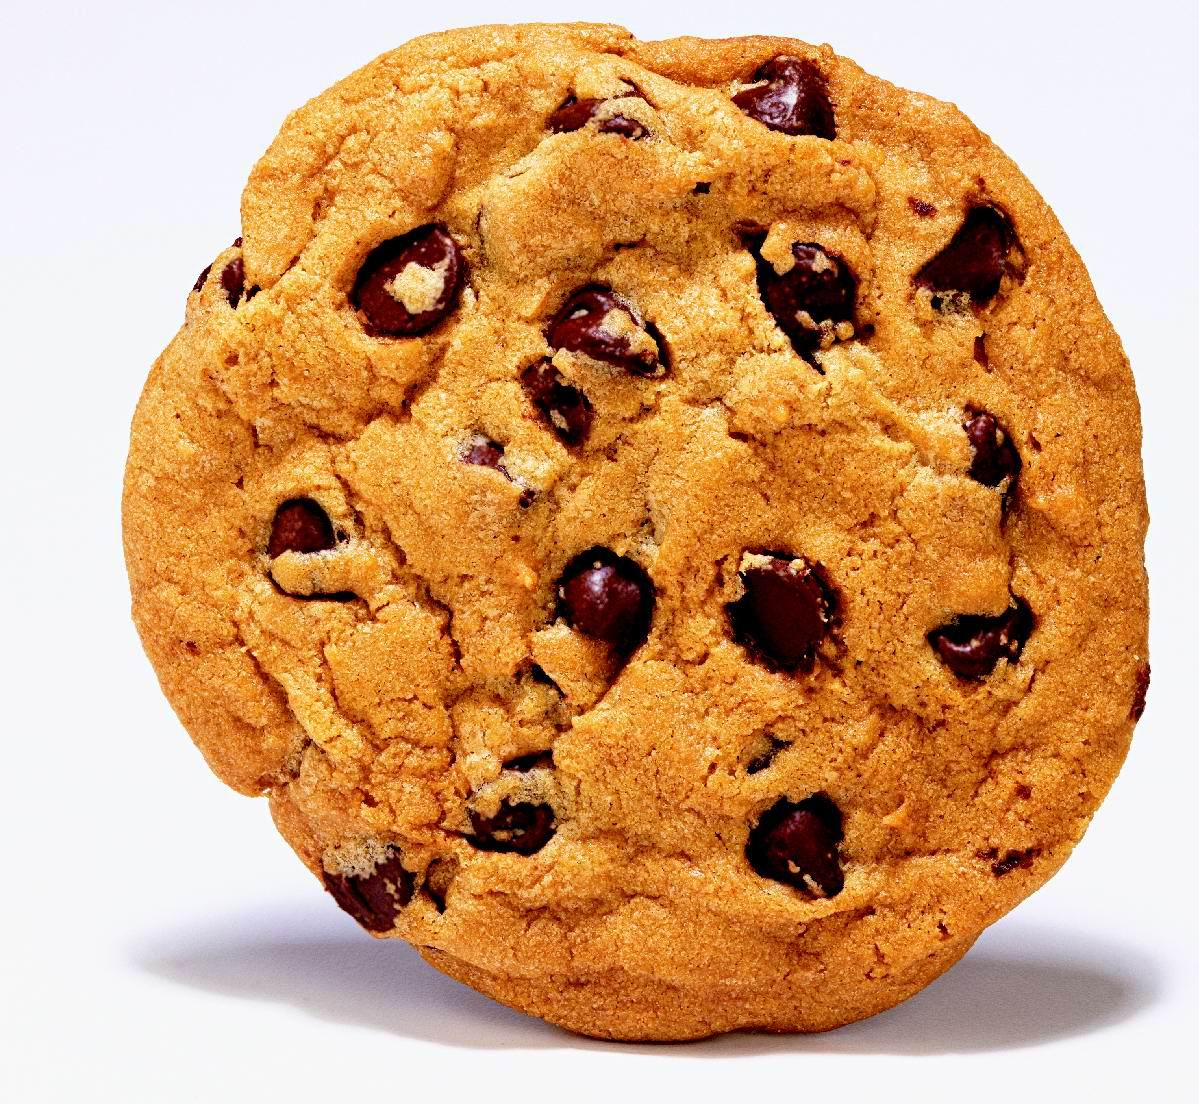
\includegraphics[height=10mm, width=10mm]{cookie.jpg}
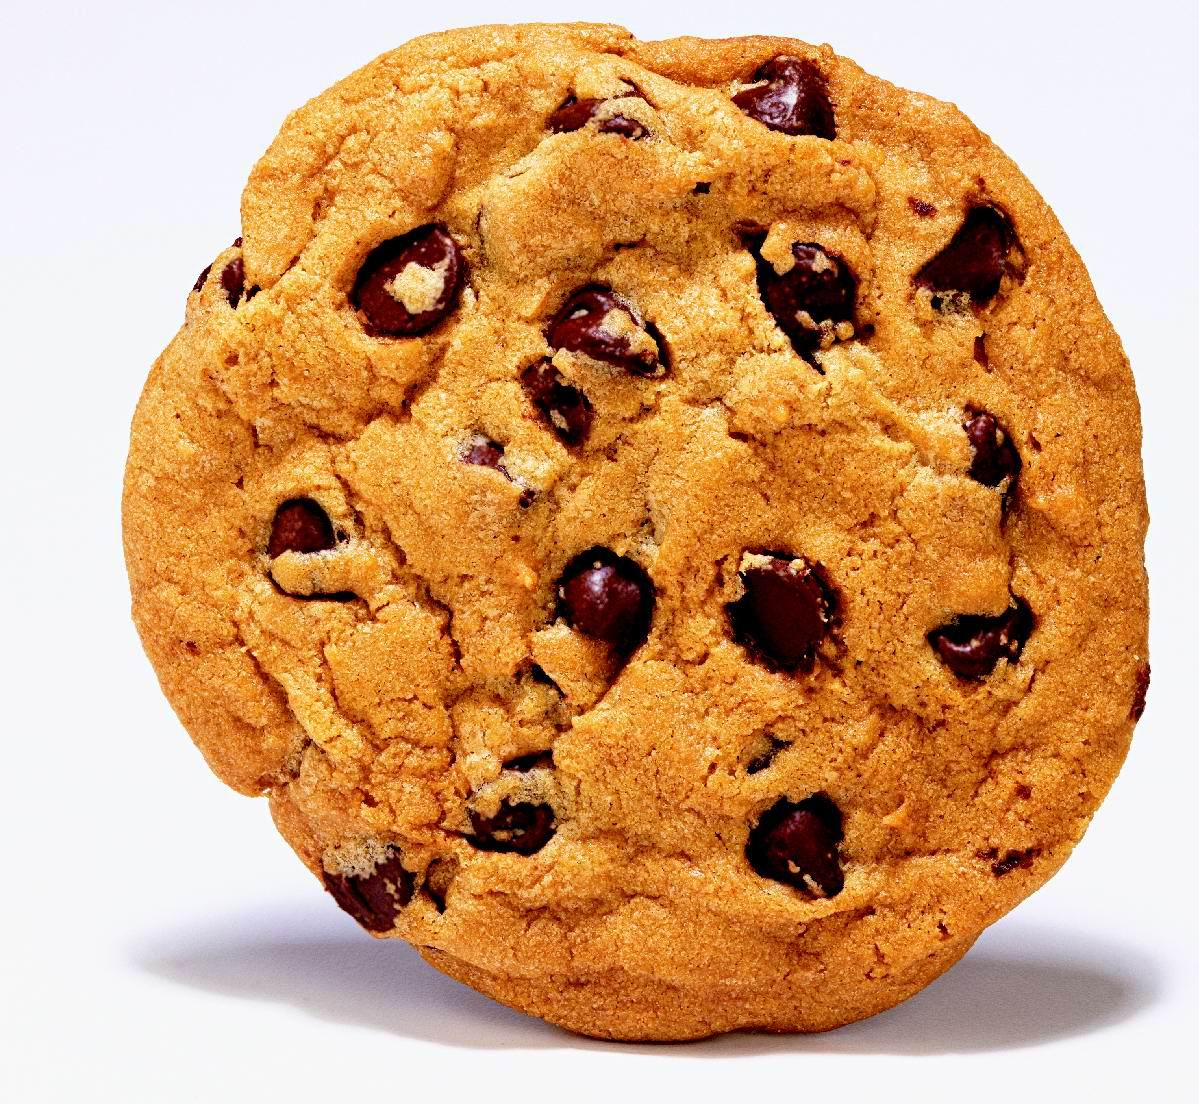
\includegraphics[height=10mm, width=10mm]{cookie.jpg}
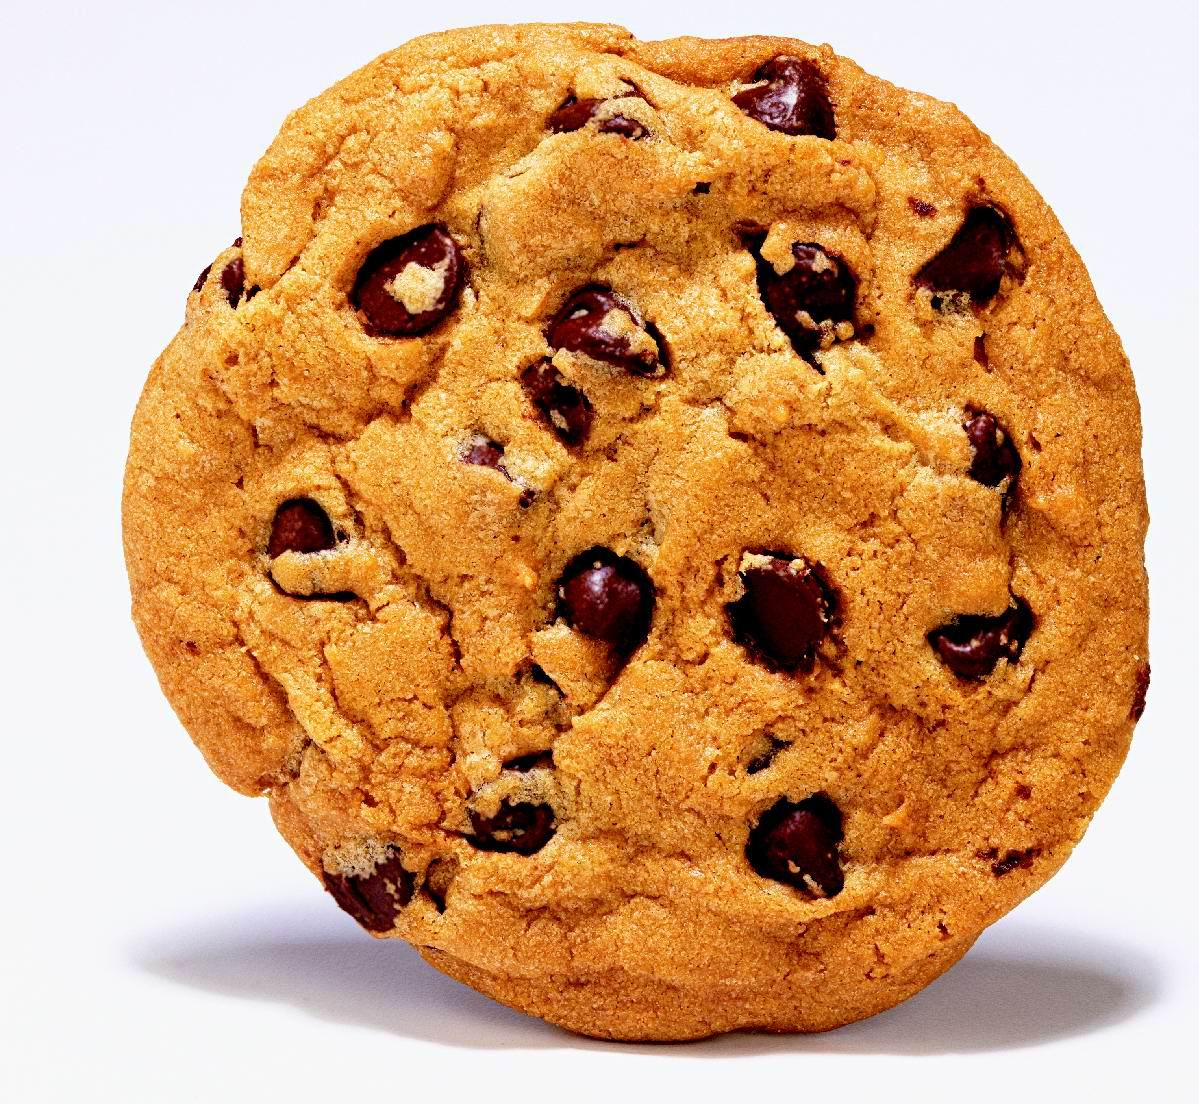
\includegraphics[height=10mm, width=10mm]{cookie.jpg}
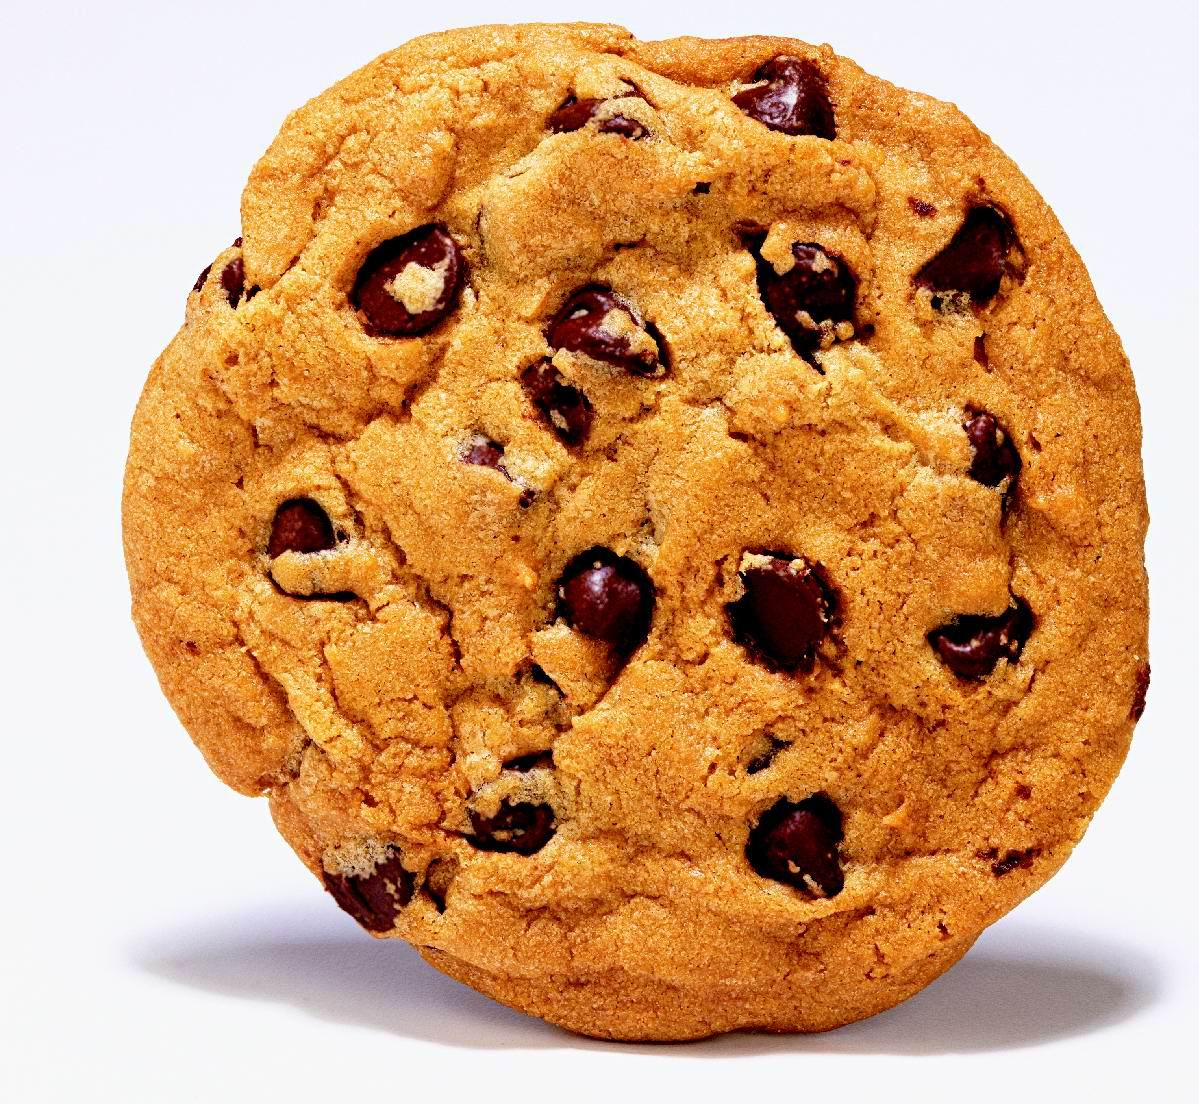
\includegraphics[height=10mm, width=10mm]{cookie.jpg}
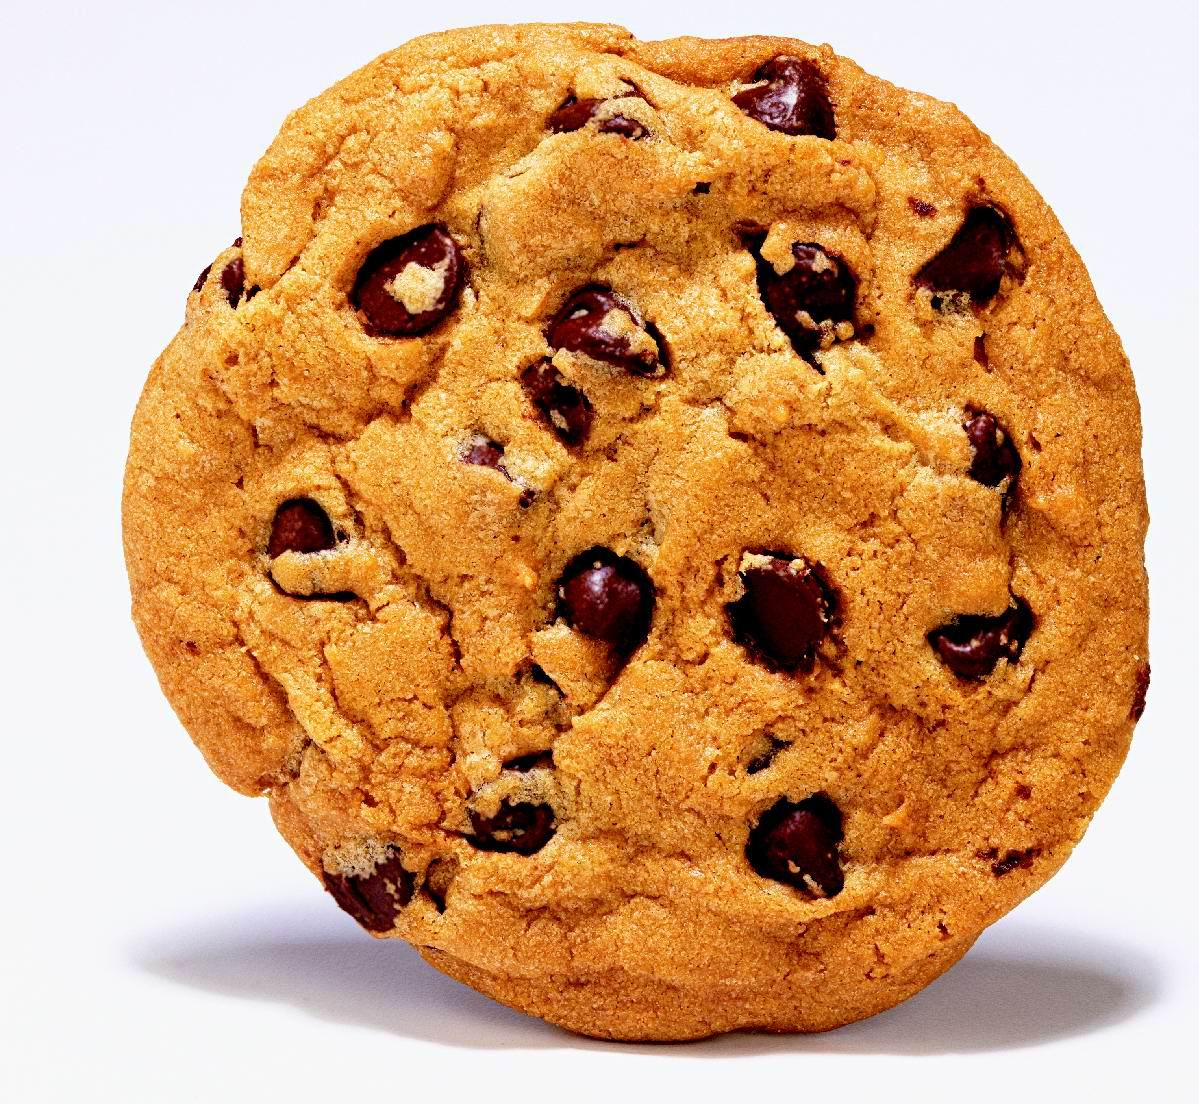
\includegraphics[height=10mm, width=10mm]{cookie.jpg}
\\
B: ``[rapid response] You gave me 11 cookies!''\\
A: ``How did you know so quickly?''\\
B: ``There's only one more than in the first batch.''\\
A: ``So you didn't recount because you remembered there were 10 in the first batch! Dynamic Programming is just a fancy way to say `remembering stuff to save time later'.''
\newpage
\section{References}

\begin{itemize}
\item Carnegie Mellon Fall 2010 15211 Fundamentals of Algorithms and Data Structures, Dr. Bill Schleris and Dr. Chris Langmead
\item Inspired by Jonathan Paulson's answer on quora:
http://www.quora.com/Computer-Programming/How-should-I-explain-dynamic-programming-to-a-4-year- old/answer/Jonathan-Paulson
\end{itemize}


\end{document}